\section{Week 3}
The convection coefficient $h$ depends on
\begin{itemize}
    \item \color{blue}Fluid properties\color{black}
    \begin{itemize}
        \item density $\rho$
        \item viscosity $\mu$
        \item thermal conductivity $k$
        \item specific heat $c_p$
    \end{itemize}
    \item \color{blue} Surface geometry
    \item Flow conditions \color{black}
    \begin{itemize}
        \item \textbf{\underline{Laminar flow:}} smooth, orderly, low velocities, high viscosity. $h$ reduces as $\delta$ increases
        \item \underline{\textbf{Transition.}} Sudden increase in $h$ due to enhanced mixing.
        \item \underline{\textbf{Turbulent flow:}} chaotic, disorganized, high velocity, low viscosity. $h$ reduces as $\delta$ continues to increase
    \end{itemize}
    \begin{figure}[H]
        \centering
        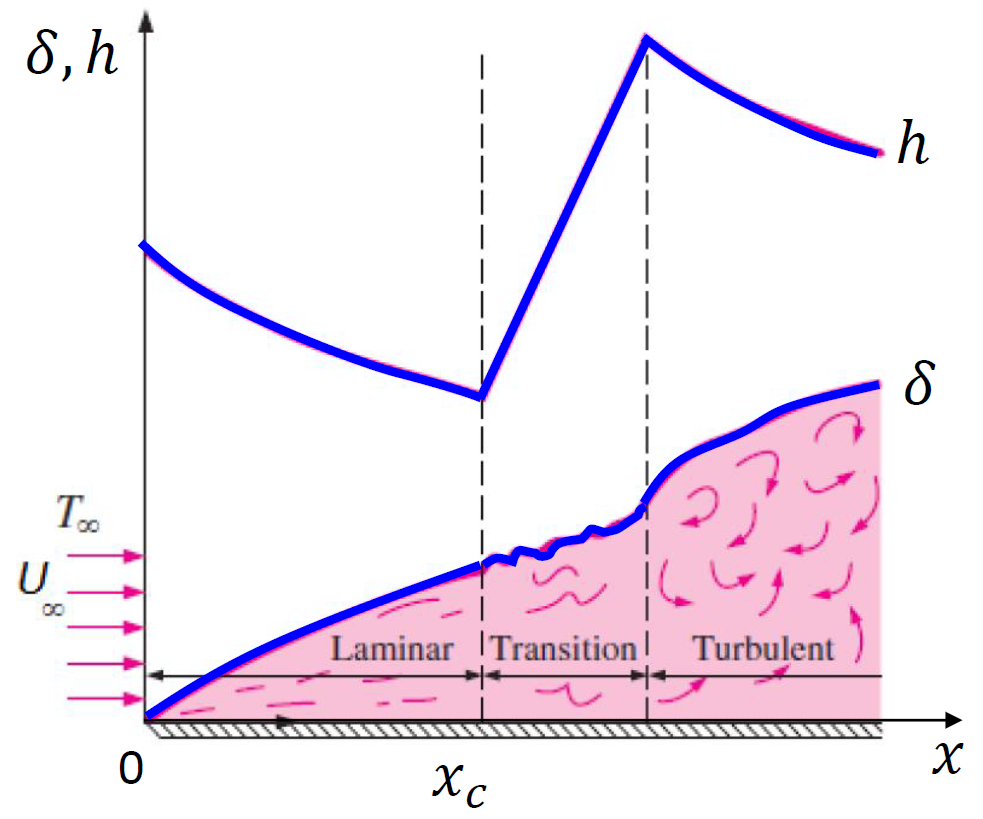
\includegraphics[width=0.8\linewidth]{images/convection_vs_Renold.png}
    \end{figure}
\end{itemize}

\underline{\textbf{\large Reynolds number:}}
\begin{figure}[H]
    \centering
    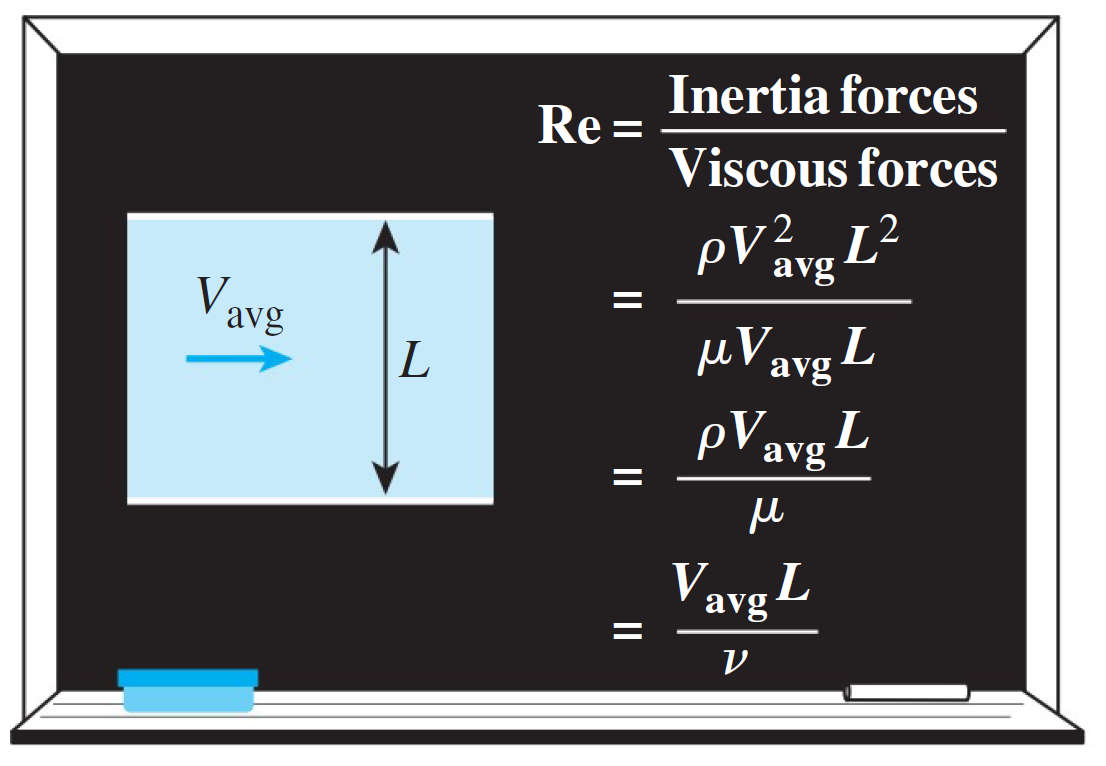
\includegraphics[width=0.8\linewidth]{images/Renolds_Number.png}
\end{figure}
\begin{itemize}
    \item Critical Reynolds number: transition from laminar to turbulent
    \begin{equation*}
        \text{Re}_{x,c} \approx 5\times 10^5
    \end{equation*}
    \begin{itemize}
        \item Transition can \color{red} be advanced \color{black} if the surface roughness is high;
        \item Transition can \color{red} be delayed \color{black} if there are suction / vortex generators 
    \end{itemize}
    \item Characteristic Length
\end{itemize}
\textbf{\underline{Prandtl Number}}
\begin{equation*}
    \text{Pr} = \frac{c_p \mu}{k} = \frac{v}{\alpha}
\end{equation*}
\begin{itemize}
    \item \color{red}Pr \color{black} is a ratio of \color{blue} momentum diffusivity \color{black} (kinematic viscosity, $v$) to \color{blue} thermal diffusivity \color{black} ($\alpha$)
    \item \color{red} Pr \color{black} is a measure of the \color{blue} relative effectiveness of momentum \color{black} and \color{blue} thermal energy transport \color{black} by diffusion in the velocity and thermal boundary layers.
    \begin{align*}
        \text{Pr} &\approx 1 \; \; \text{momentum and heat dissipation comparable} \\
        \text{Pr} &< 1 \;\; \text{heat diffuses quickly (typical in air, liquid, metals)} \\
        \text{Pr} &> 1 \;\;\text{heat diffuses slowly (typical in oils, water)}
    \end{align*}
\end{itemize}
\textbf{\underline{Principle of Similarity}}
\begin{itemize}
    \item Despite different length, different velocities, and different fluids, the two situations are compatible if $Re_1=Re_2$, $Pr_1 = Pr_2$, $Nu_1 = Nu_2$.
\end{itemize}

\textbf{\underline{Film Temperature}}
\begin{itemize}
    \item average temperature between $T_{\infty}$ and $T_{s}$: 
    \begin{equation*}
        T_f = \frac{T_{\infty}+T_{f}}{2}
    \end{equation*}
\end{itemize}

\textbf{\Large \underline{External Flow}}

\begin{itemize}
    \item Empirical form of Nußelt number: 
    \begin{equation*}
        \text{Nu}=C\cdot \text{Re}^{m}_{x}\cdot \text{Pr}^{n}
    \end{equation*}
    C, m, and n are often independent of the nature of fluid. C depends on geometry / flow.  
    \item Case 1: \color{red} Flat Plate \color{black}
    \begin{itemize}
        \item Local coefficient \color{blue} (isothermal surfaces) \color{black}
        \begin{align*}
            \text{Laminar: }\; \text{Nu} &= \frac{hx}{k} = 0.332 \text{Re}_{x}^{1/2} \text{Pr}^{1/3} \\
            Pr &> 0.6 \\
            \text{Re}_{x} &< 5\times 10^5\\
            \text{Turbulent: }\; \text{Nu} &= \frac{hx}{k} = 0.0296 \text{Re}_{x}^{0.8} \text{Pr}^{1/3} \\
            0.6 &< Pr < 60 \\
            5\times 10^5 &< \text{Re}_{x} < 10^7
        \end{align*}
        \item Average coefficient
        \begin{align*}
            \text{Laminar: }\; \overline{\text{Nu}}_L &= \frac{\bar{h}L}{k} = 0.664 \text{Re}_{L}^{1/2} \text{Pr}^{1/3} \\
            \text{Turbulent: }\; \overline{\text{Nu}}_L &= \frac{\bar{h}L}{k} = 0.037 \text{Re}_{L}^{0.8}
        \end{align*}
        \item Local coefficient \color{blue} (uniform heat flux) \color{black}
        \begin{align*}
            \text{Laminar: }\; \text{Nu} &= \frac{hx}{k} = 0.453 \text{Re}_{x}^{1/2} \text{Pr}^{1/3} \\
            Pr &> 0.6 \\
            \text{Re}_{x} &< 5\times 10^5\\
            \text{Turbulent: }\; \text{Nu} &= \frac{hx}{k} = 0.0308 \text{Re}_{x}^{0.8} \text{Pr}^{1/3} \\
            0.6 &< Pr < 60 \\
            5\times 10^5 &< \text{Re}_{x} < 10^7
        \end{align*}
        \item Flow composed of both laminar and turbulent regions:
        \begin{align*}
            \overline{\text{Nu}}_L &= \left(0.037\, \text{Re}_{L}^{4/5}-A\right)\, \text{Pr}^{1/3} \\
            A &= 0.037 \, \text{Re}^{4/5}_{x,c} - 0.664 \, \text{Re}^{1/2}_{x,c} 
        \end{align*}
        \begin{table}[H]
            \centering
            \begin{tabular}{|l|l|l|l|}
            \hline
            \textbf{$\text{Re}_{x,c}$}   & \textbf{$10^5$} & \textbf{$5\times 10^5$} & \textbf{$10^6$} \\ \hline
            $A$                          & 160             & 871                     & 1671            \\ \hline
            $\overline{\text{Nu}}_L$     & 2645            & 2014                    & 1303            \\ \hline
            $\bar{h}_L$ (W/$m^2\cdot K$) & 79.2            & 60.2                    & 39              \\ \hline
            $q'$ (W/m)                   & 17,420          & 13,270                  & 8595            \\ \hline
            \end{tabular}
        \end{table}
        \item Weighted average of surface temperature
        \begin{align*}
            \overline{T_s - T_{\infty}} &= \frac{1}{L} \int_{0}^{L} \left(T_s - T_{\infty}\right)\, dx \\
            &= \frac{q^{''}_{s}}{L} \int_{0}^{L} \frac{x}{k \text{Nu}_x} \, dx
        \end{align*}
    \end{itemize}
    \item Case 2: \color{red} Cylinder \color{black}
    \begin{align*}
        \text{Re}_D &\equiv \frac{\rho V D}{\mu} = \frac{VD}{v} \\
        \overline{\text{Nu}}_D &= \frac{\bar{h}D}{k}
    \end{align*}
    \begin{itemize}
        \item Churchill and Bernsein's equation:
        \begin{equation*}
            \text{Criterion of application:}\;\;\text{Re}\cdot \text{Pr} > 0.2
        \end{equation*}
    \end{itemize}
\end{itemize}
\begin{equation*}
            \overline{\text{Nu}}_D = 0.3 + \frac{0.62\, \text{Re}_D^{1/2}\, \text{Pr}^{1/3}}{\left(1+(\frac{0.4}{\text{Pr}})^{2/3}\right)^{1/4}} \left[1+\left(\frac{\text{Re}_D}{282000}\right)^{5/8}\right]^{4/5}
        \end{equation*}
\begin{figure}[H]
    \centering
    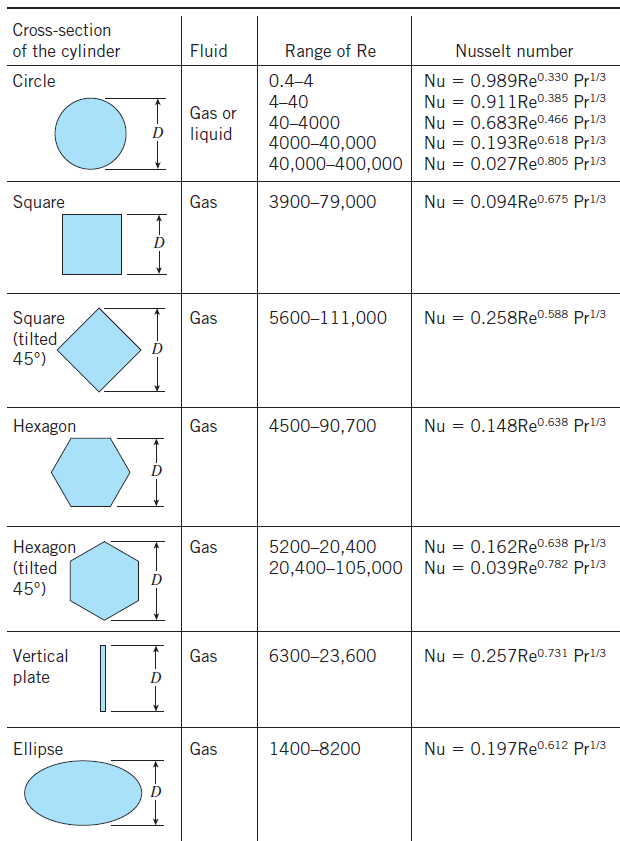
\includegraphics[width=1.0\linewidth]{images/Nusselt_Number_Cylinder.png}
\end{figure}

\begin{itemize}
    \item Case 3: \color{red} Sphere \color{black}
    
    Whitaker's correlation:
    \begin{equation*}
        \overline{\text{Nu}}_D = 2 + \left(0.4\text{Re}_{D}^{1/2}+0.06\text{Re}_{D}^{2/3}\right)\text{Pr}^{0.4}\left(\frac{\mu_{\infty}}{\mu_s}\right)^{1/4}
    \end{equation*}
    Limits of application (all properties are evaluated at $T_{\infty}$, except $\mu_s$ which is at $T_s$):
    \begin{align*}
        3.5 &< \text{Re}_D < 7.6 \times 10^5 \\
        0.71 &< \text{Pr} < 380 \\
        1 &< \frac{\mu_{\infty}}{\mu_s} < 3.2
    \end{align*}
\end{itemize}

\begin{itemize}
    \item Case 4: \color{red} Flow across tube banks \color{black}
    \begin{figure}[H]
        \centering
        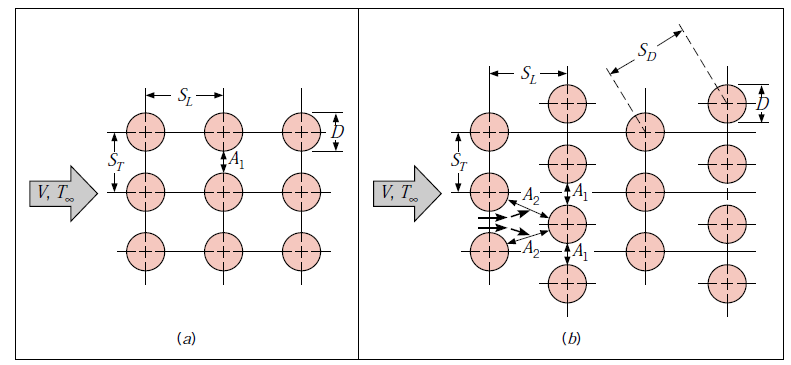
\includegraphics[width=1.0\linewidth]{images/tube_bank.png}
    \end{figure}
    \begin{itemize}
        \item Aligned:
        \begin{equation*}
            V_{max} = V \frac{S_T}{S_T-D}
        \end{equation*}
        \item Staggered:
        \begin{align*}
            V_{max} &= V \frac{S_T}{S_T - D} \; \; \text{if 2$A_2>A_1$} \\
            V_{max} &= V \frac{S_T}{2(S_D - D)}\;\; \text{if 2$A_2<A_1$}
        \end{align*}
        \item Average Nusselt Number for an isothermal array:
        \begin{align*}
            \overline{\text{Nu}}_D &= \frac{hD}{k} = C \,\text{Re}^m_D \, \text{Pr}^n \left(\frac{\text{Pr}}{\text{Pr}_s}\right)^{0.25}\\
            \text{Nu}_{D,N_{L<16}} &= F \, \text{Nu}_D
        \end{align*}
        Look up Table 7.2 to find $C$, $m$, and $n$, and look up Table 7.3 for correction factor $F$.
    \end{itemize}
\end{itemize}
\begin{figure}[H]
    \centering
    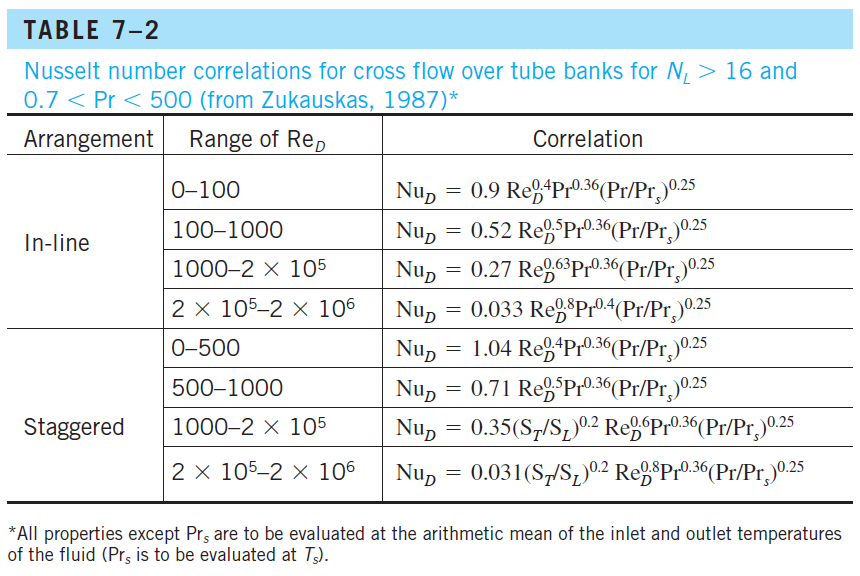
\includegraphics[width=1.0\linewidth]{images/Table_7_2.png}
    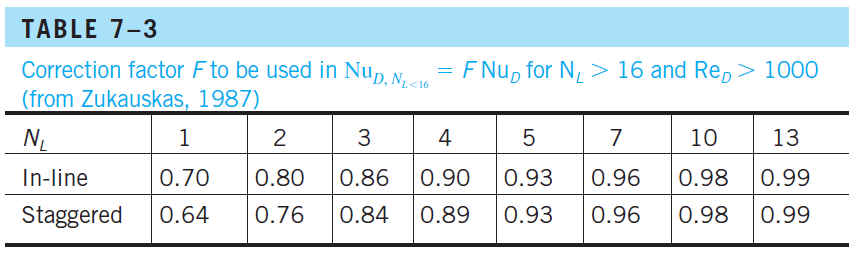
\includegraphics[width=1.0\linewidth]{images/Table_7_3.png}
\end{figure}

\underline{\textbf{\large Internal Flows}}
\begin{itemize}
    \item Hydrodynamic entrance region
    \begin{align*}
        L_{\text{h,laminar}} &\approx 0.05 \cdot \text{Re} \cdot D \\
        L_{\text{h,turbulent}} &\approx 10D
    \end{align*}
    \begin{figure}[H]
        \centering
        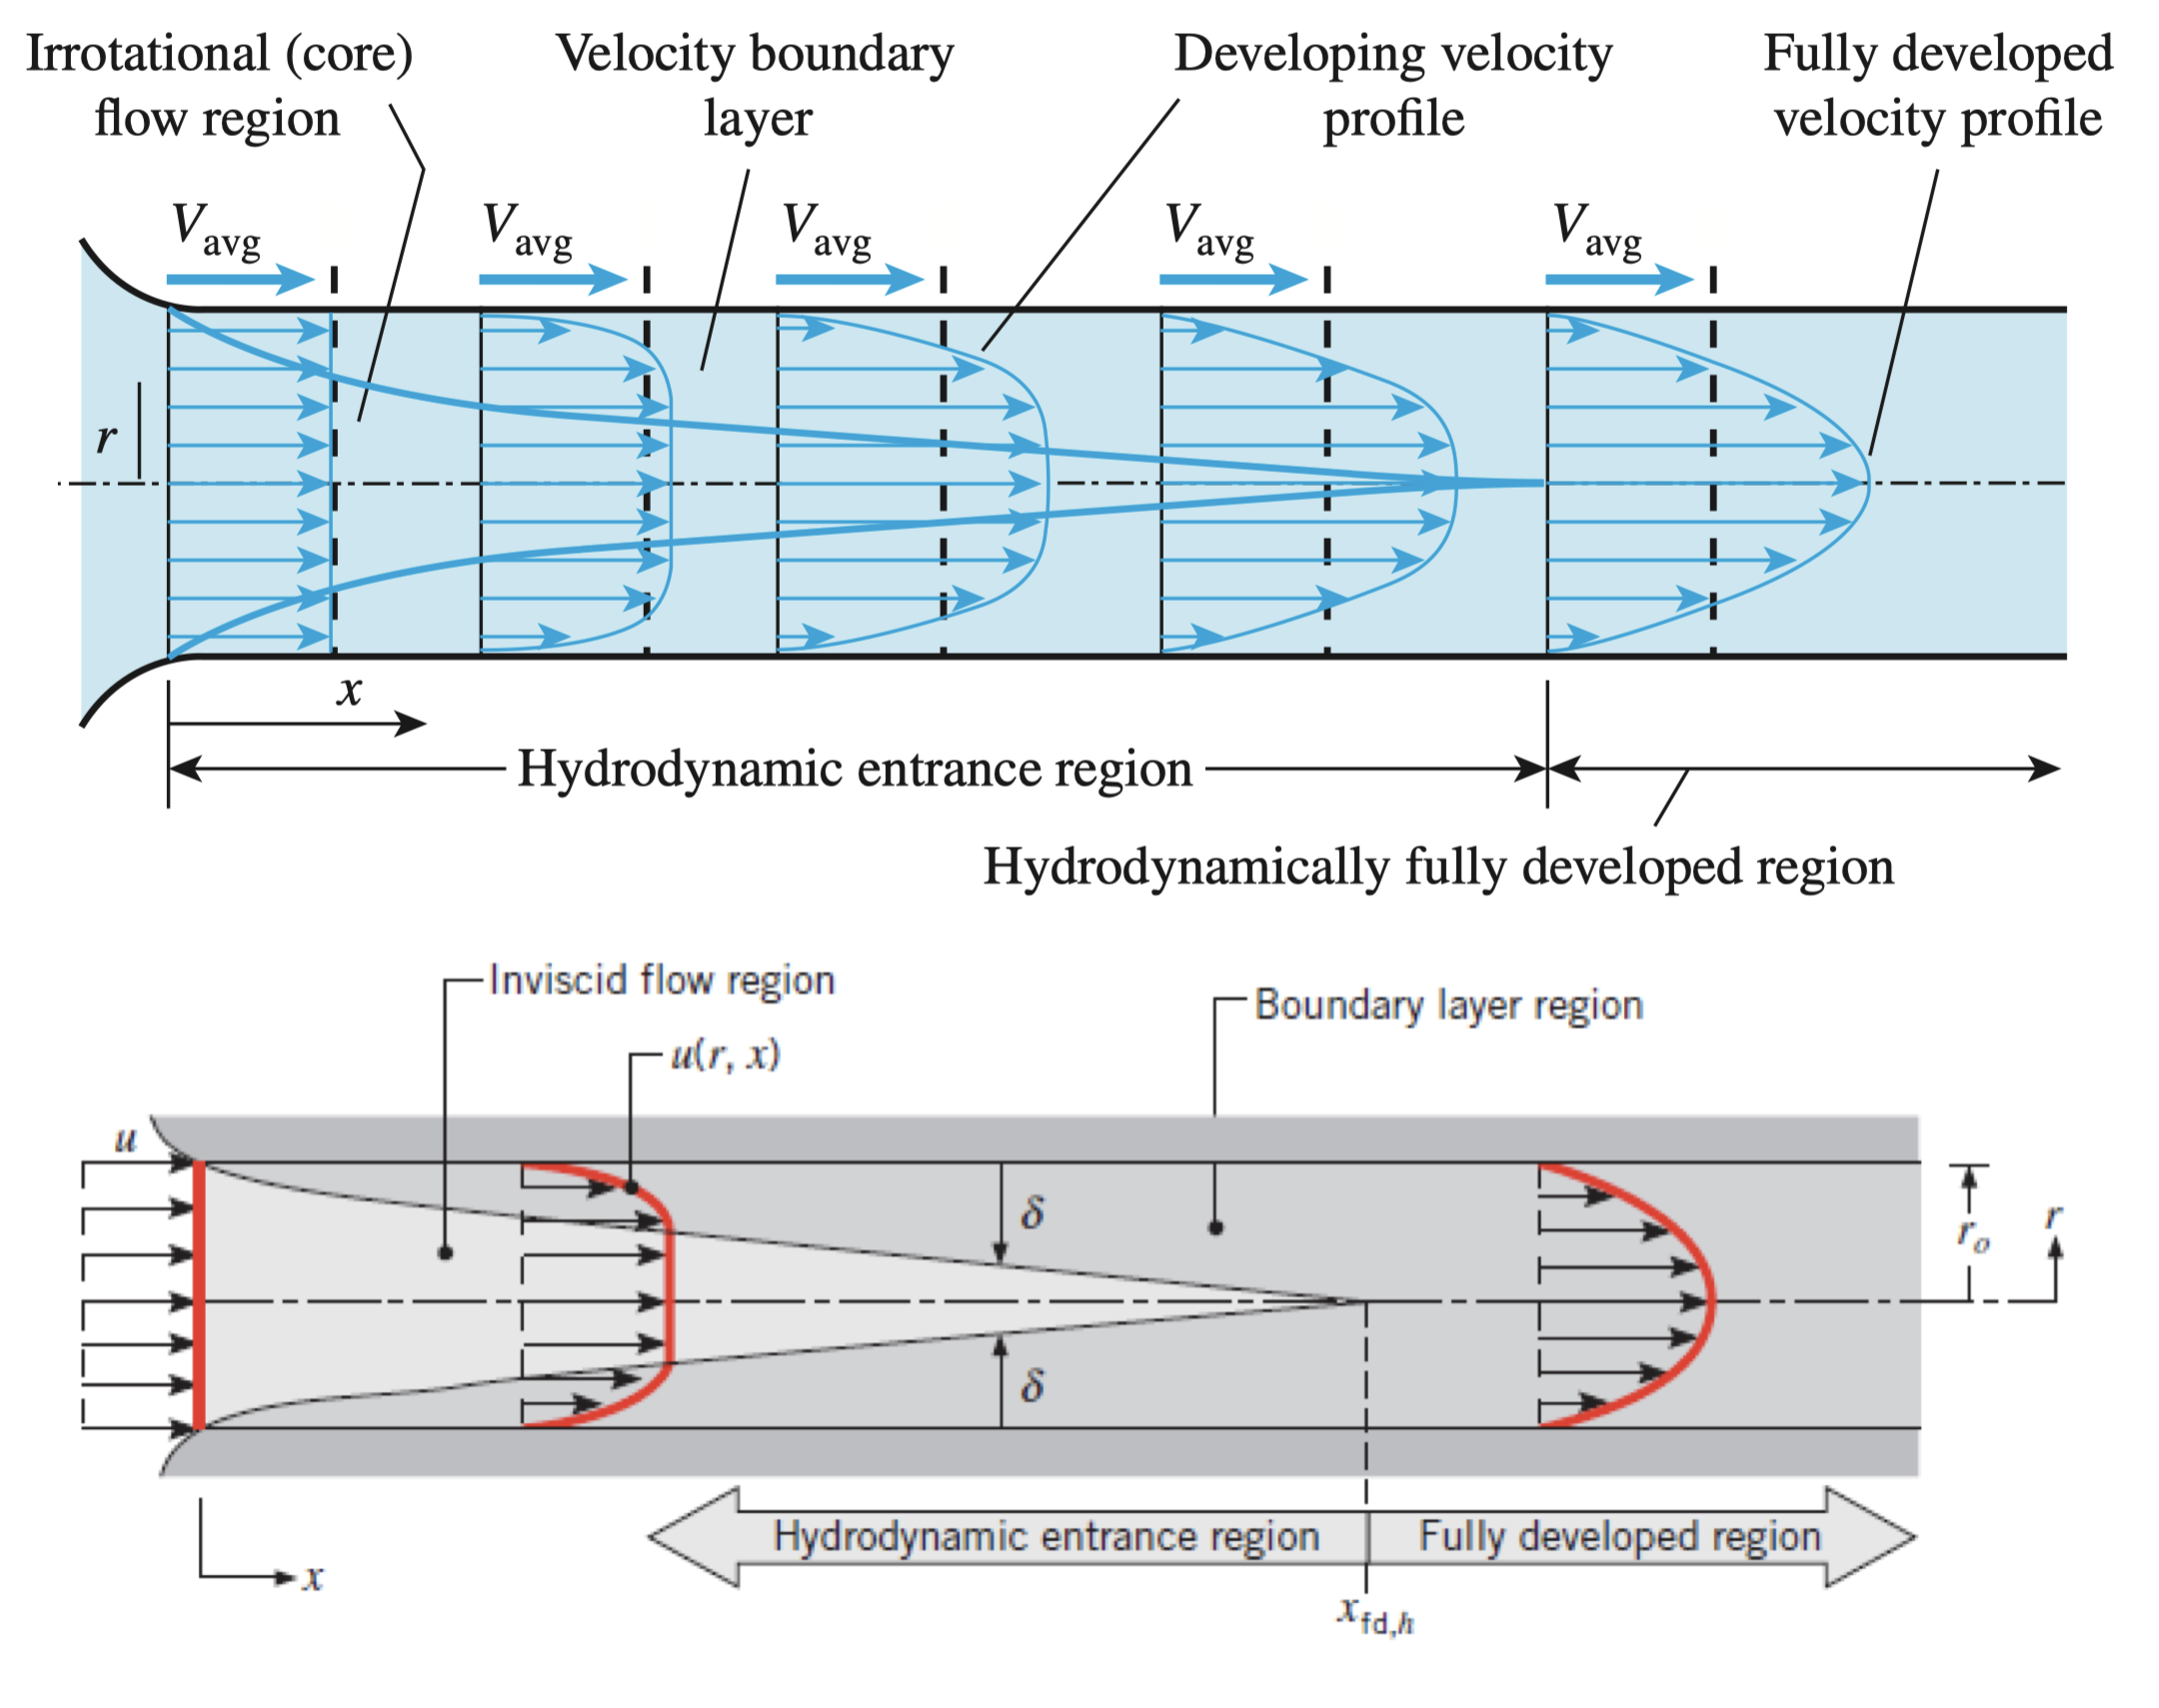
\includegraphics[width=1.0\linewidth]{images/hydrodynamic_entrance.png}
    \end{figure}
    \item Thermal entrance region
        \begin{align*}
            L_{\text{t,laminar}} &\approx 0.05 \cdot \text{Re} \cdot \text{Pr} \cdot D = \text{Pr}\cdot L_{\text{h,laminar}}
        \end{align*}
        \begin{figure}[H]
            \centering
            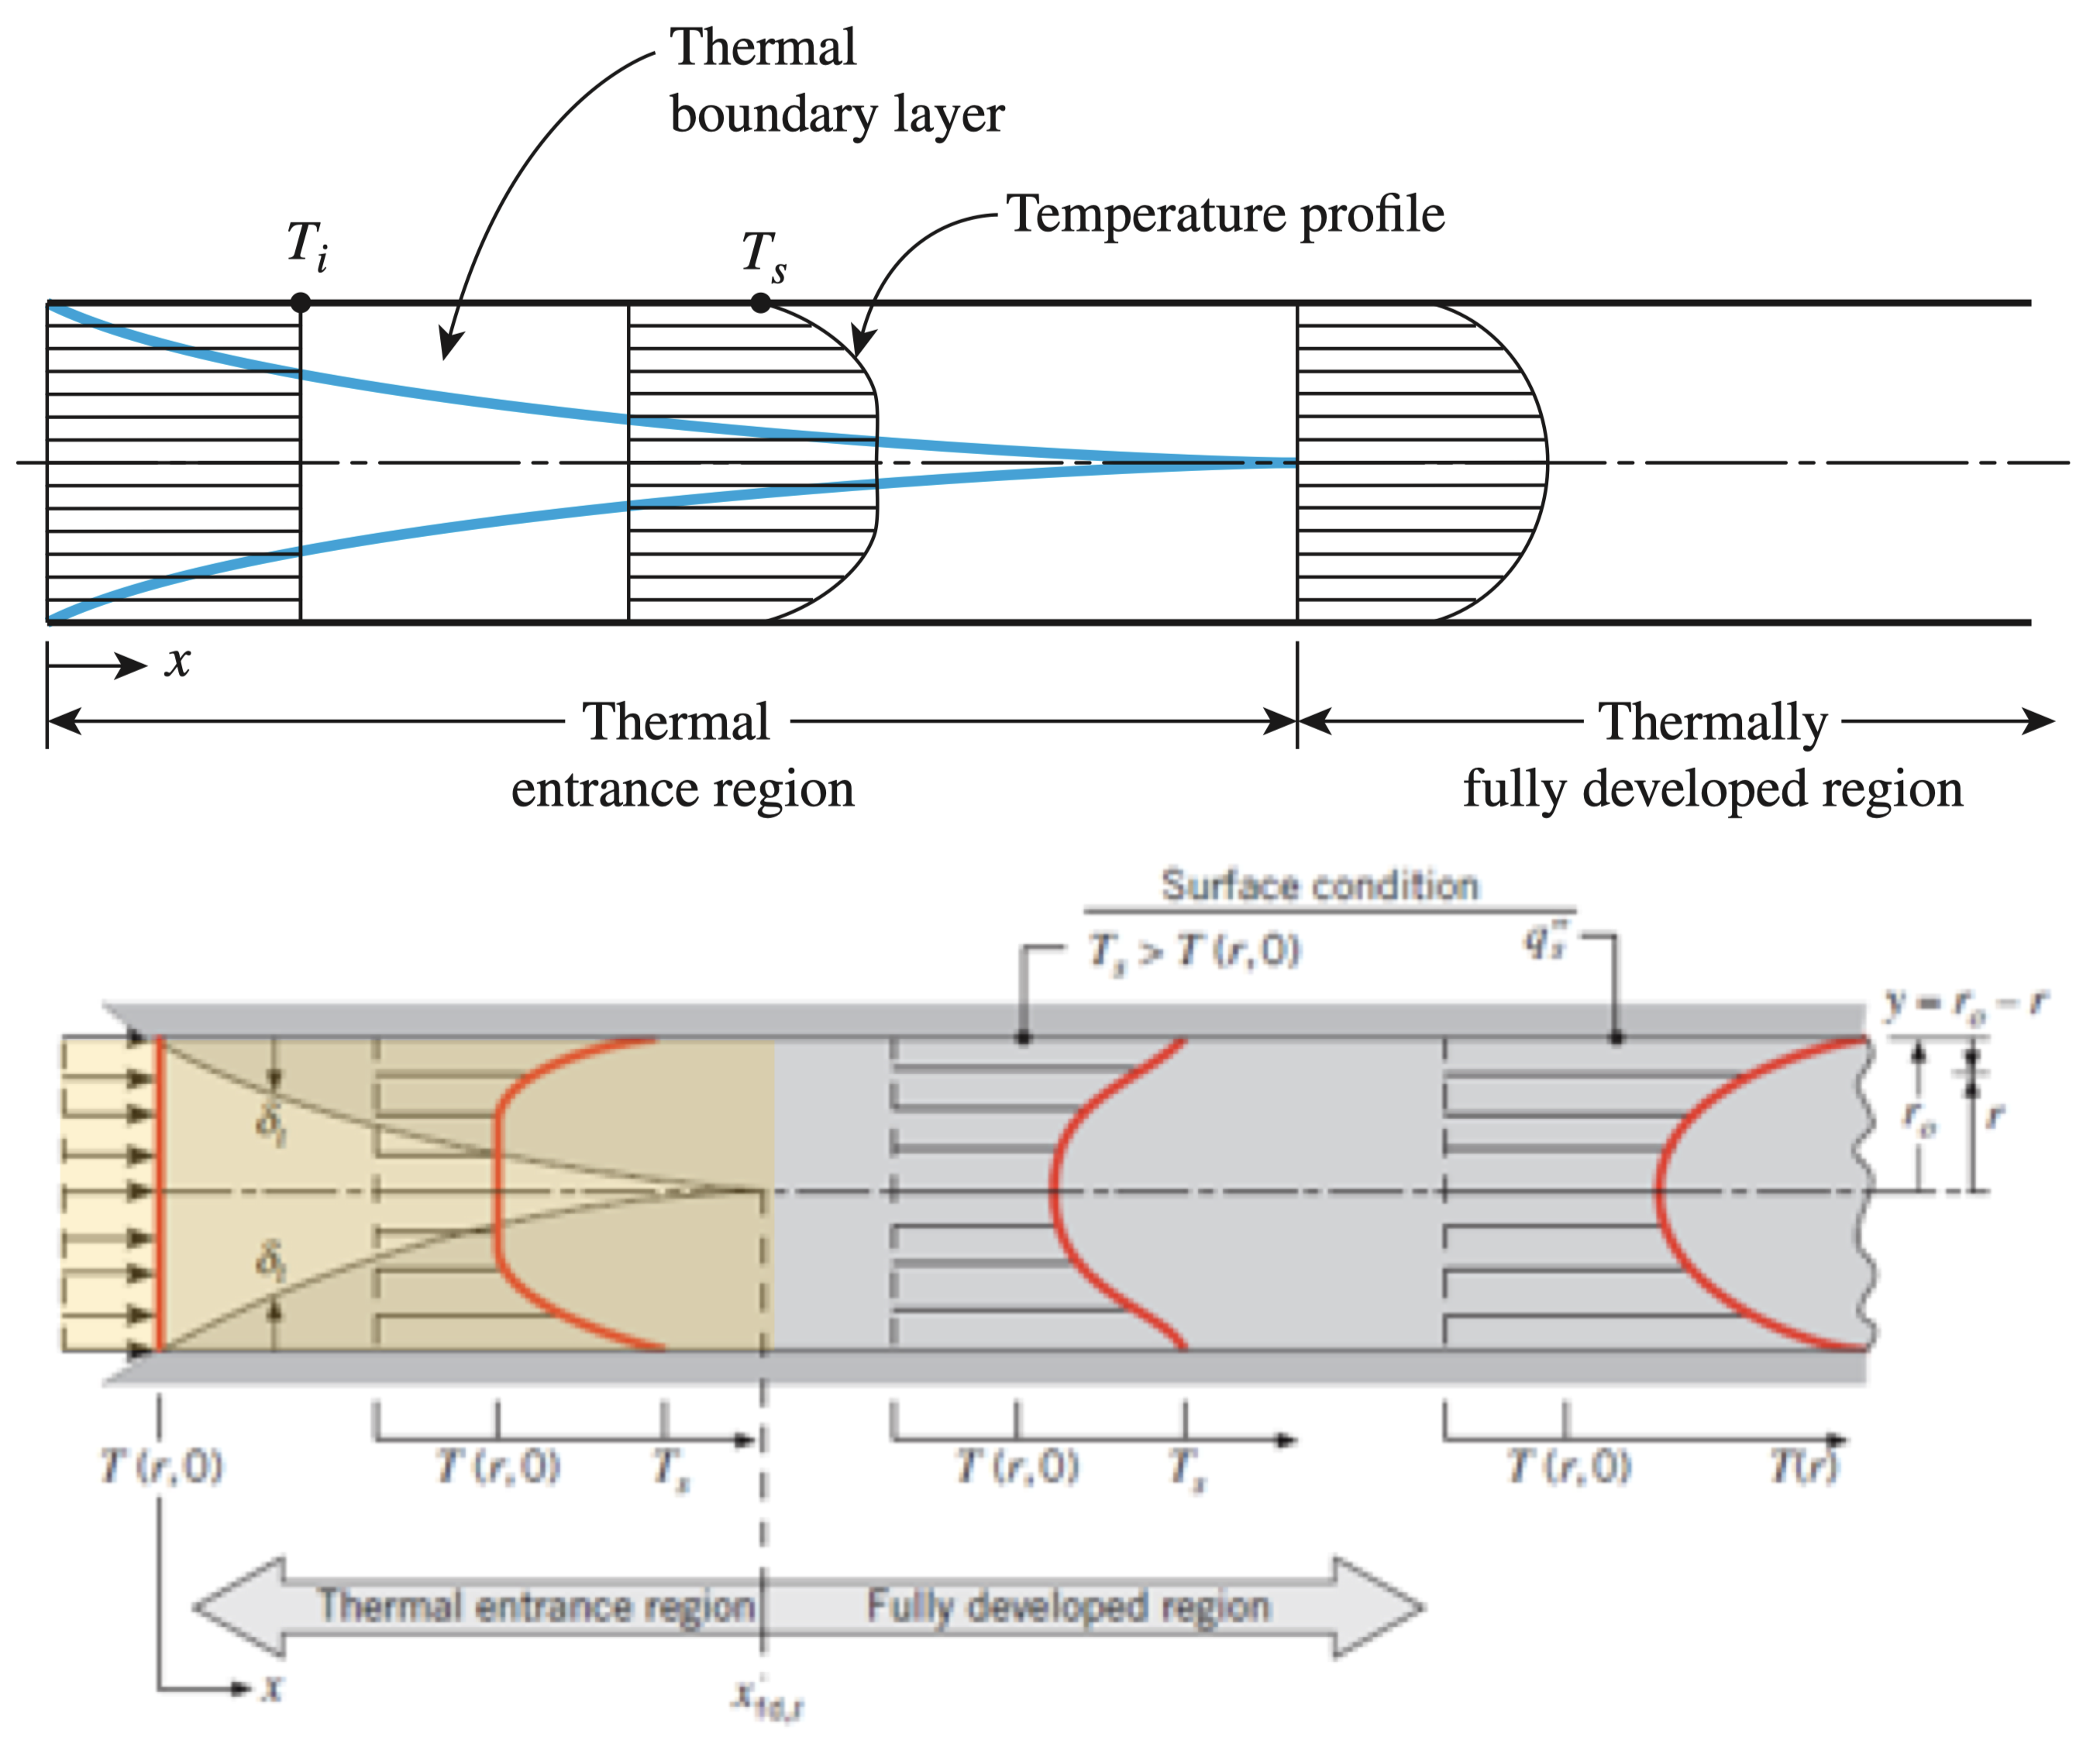
\includegraphics[width=1.0\linewidth]{images/thermal_entrance.png}
        \end{figure}
\end{itemize}
\begin{itemize}
        \item Reynolds number:
        \begin{align*}
            \text{Re}_D &= \frac{\rho u_m D_h}{\mu} \\
            \text{where } D_h &= \frac{4\cdot\text{crosssection area}}{perimeter} = \frac{4A_c}{P}
        \end{align*}
        \color{red}\underline{For a circular pipe:}\color{black}
        \begin{align*}
            \text{Re}_D &= \frac{\rho u_m D}{\mu} = \frac{\rho D}{\mu} \left(\frac{\dot{m}}{\rho (\pi D^2 /4)}\right) = \frac{4\dot{m}}{\mu \pi D}
        \end{align*}
        \item \color{red}\underline{For an annulus (ring circular pipe):}\color{black}
        \begin{equation*}
            D_h = D_o - D_i
        \end{equation*}
        \begin{align*}
            \text{Re}_D &= \frac{\rho u_m D_h}{\mu} \\
            &= \frac{\rho (D_o - D_i)}{\mu} \times \frac{\dot{m}}{\rho \pi (D_o^2 - D_i^2)/4} \\
            &= \frac{4 \dot{m}}{\pi (D_o + D_i)\mu }
        \end{align*}
        \begin{figure}[H]
            \centering
            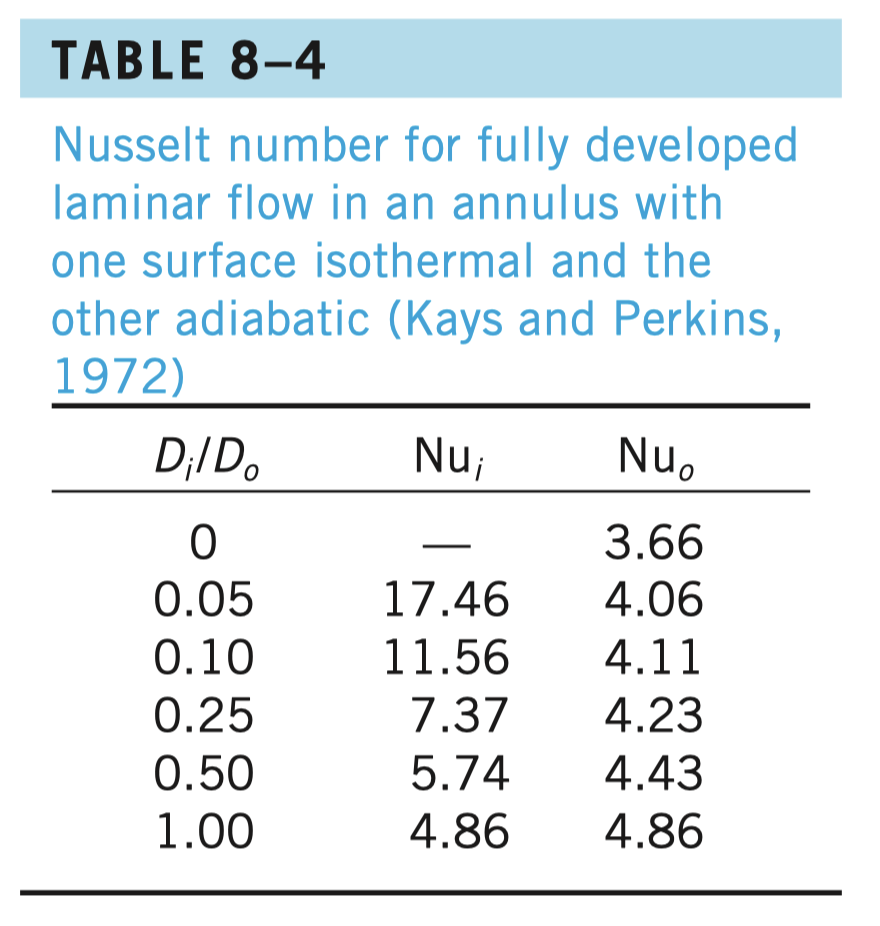
\includegraphics[width=0.7\linewidth]{images/internal_flow_annulus.png}
        \end{figure}
        \item Onset of turbulence occurs at a critical Reynolds number of:
        \begin{equation*}
            \text{Re}_{D,c} \approx 2300
        \end{equation*}
        \item Fully turbulent conditions exist for: 
        \begin{equation*}
            \text{Re}_D\approx 10000
        \end{equation*}
\end{itemize}
\textbf{\underline{\large Mean Temperature}}
\begin{itemize}
    \item Constant surface heat flux
    \begin{align*}
        \dot{Q} &= q^{''}_{s}A_s = \dot{m} c_p (T_e - T_i) \\
        T_m &= T_i + \frac{P q_{s}^{''}}{\dot{m}c_p} x \\
        T_s &= T_m + \frac{q_{s}^{''}}{h}
    \end{align*}
    \item Constant surface temperature
    \begin{align*}
        \Delta T &\equiv T_s - T_m \\
        \Delta T_{lm} &= \frac{\Delta T_e - \Delta T_i}{\ln(\Delta T_e / \Delta T_i)} \\
        \dot{Q} &= \overline{h} A_s \Delta T_{lm}
    \end{align*}
    where $\Delta T_{lm}$ is the log-mean temperature difference.
\end{itemize}

\textbf{\underline{\large Fully Developed Flow}}
\begin{itemize}
    \item For hydraulically and thermally fully-developed \color{blue} laminar flow \color{black} in a \color{blue} circular tube \color{black}:
    \begin{enumerate}
        \item Constant surface heat flux $q_{s}^{''}$:
        \begin{equation*}
            \text{Nu}_D = \frac{hD}{k} = 4.36 \; \; \text{constant everywhere}
        \end{equation*}
        \item Constant surface temperature $T_s$:
        \begin{equation*}
            \text{Nu}_D = \frac{hD}{k} = 3.66 \;\;\text{constant everywhere}
        \end{equation*}
    \end{enumerate}
    \begin{figure}[H]
            \centering
            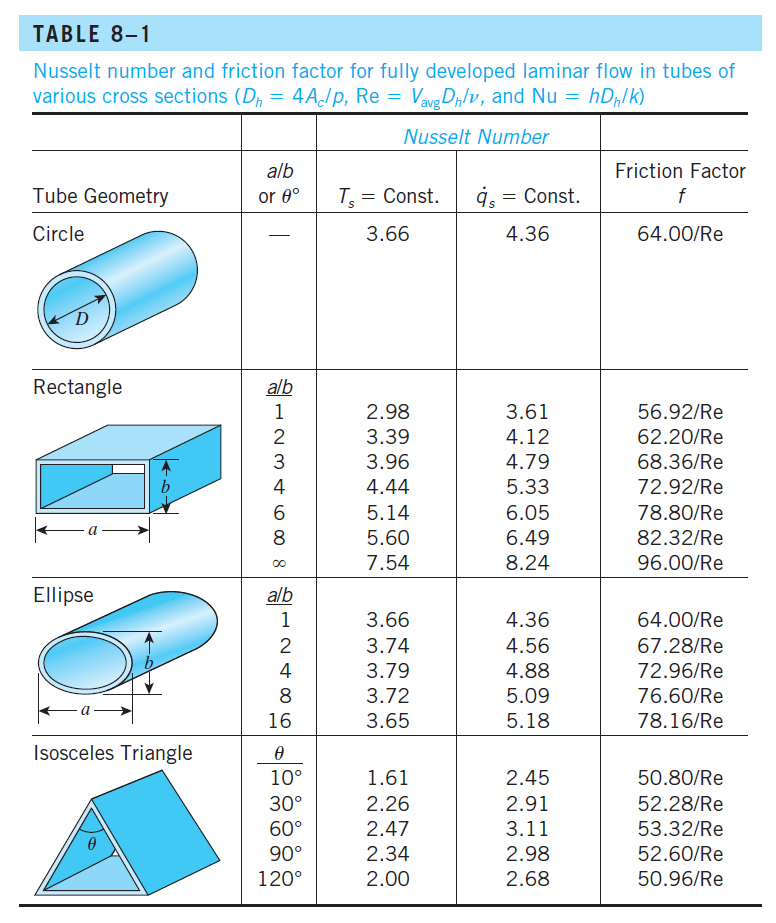
\includegraphics[width=1.0\linewidth]{images/Table_8_1.png}
    \end{figure}
    Note: to determine $h$, evaluate $k$ at $T_m$
    \item For  hydraulically and thermally fully-developed \color{blue} turbulent flow \color{black} in a \color{blue} circular tube \color{black}:
    \begin{enumerate}
        \item For a smooth surface and fully turbulent conditions:
        \begin{align*}
            \text{Nu}_D &= 0.023 \, \text{Re}_D^{4/5} \, \text{Pr}^n \\
            \text{where } n &= 0.3 \; \text{ if } T_s < T_m \\
            n &= 0.4 \; \text{ if } T_s > T_m 
        \end{align*}
        Criteria of application:
        \begin{align*}
            0.6 &	\lesssim \text{Pr} 	\lesssim 160 \\
            \text{Re}_D &\gtrsim 10000 \\
            \frac{L}{D} &\gtrsim 10
        \end{align*}
    \end{enumerate}
\end{itemize}
